% !TEX program = XeLaTeX
% !TEX encoding = UTF-8
\documentclass[UTF8,nofonts]{article}

\usepackage{kotex}
\usepackage{url}
\usepackage{cancel}
\usepackage{xspace}
\usepackage{graphicx}
\usepackage{multicol}
\usepackage{multirow}
\usepackage{subfig}
\usepackage{amsmath}
\usepackage{amssymb}
\usepackage[a4paper, width=186mm, top=18mm, bottom=18mm, includeheadfoot]{geometry}
%\usepackage[a4paper, width=140mm, top=18mm, bottom=22mm, includeheadfoot]{geometry}
\usepackage{booktabs}
\usepackage{array}
\usepackage{verbatim}
\usepackage{caption}
\usepackage{natbib}
\usepackage{booktabs}
\usepackage{float}
\usepackage{pdflscape}
\usepackage{mathtools}
\usepackage[usenames, dvipsnames]{xcolor}
\usepackage{afterpage}
\usepackage{pgf}
\usepackage{tikz}
\usepackage{dirtree}
\usepackage[style=american]{csquotes}
\usepackage{amsfonts}
\usepackage{tikz}
\usepackage{tkz-graph}
\usetikzlibrary{arrows,decorations.pathmorphing,automata,positioning,backgrounds,fit,shapes.symbols,chains,intersections}

\newtheorem{definition}{정의}[section]
\newtheorem{theorem}{Theorem}[section]
\newtheorem{lemma}{Lemma}
\newtheorem{proof}{Proof} [section]



\usepackage[toc, page, title, titletoc, header]{appendix}
\usepackage{marginnote}
\usepackage{tablefootnote}

\renewcommand\abstractname{Abstract}


\usepackage{perpage} %the perpage package
\MakePerPage{footnote} %the perpage package command

\usetikzlibrary{shapes.geometric}%
\usepackage{color}
\usepackage{eso-pic}
\usepackage[final]{pdfpages}

\hyphenpenalty=750

\title{\textbf{루프링:}\\\textbf{분권형 토큰 거래소 프로토콜}}
\author{
  Daniel Wang\\
  \texttt{daniel@loopring.org}\\
  \and
  	Jay Zhou\\
  	\texttt{jay@loopring.org}\\
  	\and
  	Alex Wang\\
  	\texttt{alex@loopring.org}\\
  	\and
  	Matthew Finestone\\
  	\texttt{matt.finestone@gmail.com}\\ 
  \\
  \texttt{https://loopring.org}
 }

\makeatletter
\def\CTEX@section@format{\Large\bfseries}
\makeatother

\makeatletter
\newenvironment{tablehere}
 {\def\@captype{table}}
 {}

\newenvironment{figurehere}
 {\def\@captype{figure}}
 {}
\makeatother

\begin{document}

\maketitle


\begin{abstract}
루프링(Loopring)은 분권형 거래소를 구축하기 위한 개방형 프로토콜입니다. 루프링은 거래와 정산을 담당하는 공개형 스마트 계약 집합으로 운영되며 오프 체인(off-chain)에서 주문을 집계하고 전달하는 행위자(actors) 그룹과 함께 운영됩니다. 프로토콜은 무료이고, 확장 가능하며, 거래소 기능을 포함한 분권형 애플리케이션(dApps)을 위해 표준화된 블록 구성을 제공합니다. 루프링의 상호 운용 가능한 표준은 무신뢰(trustless, 제삼자의 도움 없이 서로 믿고 거래 가능한) 익명 거래를 쉽게 합니다. 루프링이 기존 분권형 거래소 프로토콜보다 가장 개선된 점은 서로 다른 주문들을 조합해 주문을 만드는 능력입니다. 루프링은 2개의 토큰 페어(pair) 거래에 대한 제약을 제거하고 유동성을 획기적으로 개선했습니다. 또한, 루프링은 선행매매(front-running) - 트랜잭션을 기존 솔루션 제공자보다 빠르게 블록에 전송하려는 불공정한 시도 - 를 방지하기 위해 견고한(robust) 고유 솔루션을 사용합니다. 루프링은 블록체인에 범용적이기 때문에 스마트 계약 기능을 가진 모든 블록체인 위에 배포할 수 있습니다. 이 글이 작성된 시점을 기준으로 루프링은 이더리움(Ethereum) \cite{buterin2017ethereum} \cite{wood2014ethereum} 과 퀀텀(Qtum) \cite{dai2017smart}에서 운영할 수 있으며 네오(NEO) \cite{atterlonn2018distributed}에 대해서는 개발이 진행 중입니다. 
\end{abstract}



\begin{multicols}{2}
\section{소 개\label{sec:introduction}}

블록체인 기반 자산의 확산으로 거래 당사자들 사이에서 이들 자산을 교환하기 위한 수요가 많이 증가했습니다. 전통적인 자산에 대한 토큰화를 비롯해 수많은 새로운 토큰의 유입으로 인해 이러한 수요는 더욱 커졌습니다. 투기 거래 목적의 토큰 교환이든 네이티브 유틸리티 토큰을 사용해 이들의 네트워크에 접근하기 위한 교환이든 하나의 암호 자산을 다른 것으로 바꾸는 능력은 생태계 확장에 기본적인 요소입니다. 확실히 자산에는 잠재적인 에너지가 있으며, \cite{desotocapital}, 이 자산을 현금화하기 위해서는 - 자금 유입을 통해 - 모든 블록체인에서 제공하는 소유권 행사뿐만 아니라 자산을 자유롭게 이체하고 교환할 수 있는 능력이 필요합니다.

토큰(가치)의 무신뢰 교환의 경우 주목할만한 블록체인 기술 사용 사례(use case)입니다. 하지만, 지금까지는 암호 자산 애호가들이 주로 전통적인 중앙집권형 거래소에서 토큰 거래를 정산하고 있습니다. 비트코인이 \cite{nakamoto2008bitcoin} P2P 전자화폐에 관해 \enquote{믿을 수 있는 제삼자가 이중 지급을 방지하기 위해 여전히 필요하다면 주요 이점은 사라진다고} 충실하게 강조했듯이, 분권형 자산이 제삼자와의 신뢰 관계가 형성되어 있고, 폐쇄적이며(gated), 중앙화된 거래소를 이용해야 한다면 이들의 주요 이점이 없어지기 때문에 루프링 프로토콜이 필요합니다.

분권형 토큰을 중앙집권형 거래소에서 거래하는 것은 분권형 프로젝트가 지지하는 덕목과 맞지 않기 때문에 철학적인 관점에서 말이 되지 않습니다. 또한, 중앙집권형 거래소를 사용하는 것은 현실적인 위험과 제한이 많고 이 문제는 아랫부분에서 다루고 있습니다. 분권형 거래소 (DEXs) \cite{schuh2015bitshares} \cite{bancor} \cite{kyber}는 이러한 문제를 해결하기 위해 노력했고 대부분이 금융 직거래(disintermediation)를 위해 블록체인을 사용함으로써 보안 위험을 줄이는 데 성공했습니다. 하지만, 새로운 경제에서 DEX 역량이 매우 중요한 인프라이기 때문에 상당한 성능 향상이 필요합니다. 루프링은 dApp 범용적인 개방형 프로토콜로 인프라를 위한 모듈식 도구를 제공하는 것을 목표로 합니다.

\section{거래소의 현주소 진단\label{sec:current_exchange_landscape}}

\subsection{중앙집권형 거래소의 단점}
중앙집권형 거래소의 주요 위험 요소는 크게 세 가지입니다; 1) 보안성 부족, 2) 투명성 부족, 3) 유동성 부족.

\textbf{보안성 부족}은 사용자가 개인키(자금)에 대한 통제권을 중앙집권형 거래소에 넘겨주었기 때문에 발생합니다. 중앙집권형 거래소는 악의적인 해커의 표적이 될 가능성이 있기 때문에 사용자는 위험에 노출됩니다. 모든 중앙집권형 거래소가 직면한 보안과 해킹 위험은 잘 알려졌지만 \cite{coincheckhack}  \cite{mcmillan2014inside}, 토큰 거래를 위해서 \enquote{어쩔 수 없이 감당해야 하는 것(table stakes)}으로 여깁니다. 서버에서 수백만 달러의 고객 자금을 관리하는 한 중앙집권형 거래소는 해커에게 여전히 매력적인 공격 대상입니다. 거래소에 근무하는 개발자 역시 고객의 자금으로 장난을 칠 수 있습니다. 간단히 말하자면, 사용자가 중앙집권형 거래소에 토큰을 입금하는 순간 사용자는 자신이 소유한 토큰에 대한 통제권을 잃게 됩니다.

\textbf{투명성 부족}은 불공평하게 행동하는 부정직한 거래소의 위험에 사용자를 노출합니다. 사용자는 중앙집권형 거래소에서 실제로 자신이 소유한 토큰을 거래하는 것이 아니라 IOU(차용증서)를 거래하기 때문에 거래소 운영자가 악의적인 목적을 가지고 있다면 문제가 될 수 있습니다. 토큰을 거래소의 지갑으로 전송하면 거래소는 해당 토큰을 보관 처리하고 토큰 대신 IOU를 제공합니다. 이후, 모든 거래는 사용자 간의 IOU 사이에서 효과적으로 이루어집니다. 토큰 인출의 경우, 사용자는 거래소를 통해 IOU를 토큰으로 교환하여 사용자의 외부 지갑 주소로 받습니다. 이 과정에는 투명성이 빠져 있고, 거래소는 운영을 중단하거나, 이용자 자산을 동결할 수도 있고, 파산될 수도 있습니다. 또한, 거래소가 사용자의 토큰을 보관하는 동안, 제삼자에게 자산을 빌려주는 업무에 거래소가 보관 중인 사용자의 자산을 사용할 가능성도 있습니다. 모든 자금을 잃어버릴 수 있는 위험성뿐만 아니라 투명성 부족은 높은 거래 수수료, 수요가 최고조일 때 지연 현상 발생, 규제 리스크, 선행매매 등의 비용을 사용자에게 부과합니다.

\textbf{유동성 부족.} 거래소 운영자의 관점에서 보면, 두 가지 승자 독식 시나리오로 인해 분열된(fragmented) 유동성은 새로운 거래소의 진입을 막습니다. 첫째, 거래할 수 있는 페어 (trading pairs) 종류가 많은 거래소가 승리합니다. 사용자는 모든 거래를 거래소 한 곳에서 처리하는 것을 선호하기 때문입니다. 둘째, 주문 집계장(order book)이 가장 큰 거래소가 승리합니다. 각각의 페어 거래에서 매수매도 스프레드(spread)는 주문 집계장이 큰(매수매도 주문이 많은) 곳이 유리하기 때문입니다. 이러한 구조로 인해 초기 유동성을 만들어 내는 것이 어려운 새로운 거래소는 경쟁에서 밀리게 됩니다. 그 결과, 사용자들의 불평과 주요 해킹 사고에도 불구하고 많은 거래소가 높은 시장 점유율을 차지하게 되었습니다. 중앙집권형 거래소의 시장 점유율이 높아짐에 따라, 해킹 대상이 될 가능성도 커졌다는 점을 말해두고 싶습니다.

사용자의 관점에서 보면, 분열된 유동성은 사용자의 경험을 많이 감소시킵니다. 중앙집권형 거래소 사용자는 거래소가 보유한 유동성 풀(pool) 안에서 그들이 제공하는 호가 정보를 이용해 거래소가 지원하는 토큰 페어만 거래할 수 있습니다. 토큰 \verb|A|를 토큰 \verb|B|와 거래하려면 사용자는 두 토큰을 모두 지원하는 거래소를 방문하거나 개인 정보를 제공해 다른 거래소에 가입해야 합니다. 사용자는 BTC나 ETC에 대해 예비 거래 또는 중간 거래를 자주 실행해야 하며 이 과정에서 매수매도 스프레드를 지급해야 합니다. 마지막으로, 주문 집계장에 가격 조정 없이 거래를 체결할 수 있을 만큼 충분한 매수매도 주문이 존재하지 않을 수 있습니다. 거래소가 많은 거래량을 처리하고 있다고 주장하더라도 이 거래량과 유동성이 가짜 \cite{fakevolume}가 아니라는 보장이 없습니다.         

그 결과 유동성이 단절되고 분열된 생태계가 되었고 기존 금융 시스템과 유사하게 대부분의 거래량이 소수의 거래소에 집중됩니다. 중앙집권형 거래소 체계 안에서 블록체인의 글로벌 유동성에 대한 약속은 아무런 가치가 없습니다.  

\subsection{분권형 거래소의 단점}
분권형 거래소는 중앙집권형 거래소와 약간 차이가 있습니다. 분권형 거래소에서는 근원(underlying) 블록체인 위에서 거래를 직접 수행하기 때문에 사용자가 개인키(자산)에 대한 통제권을 가지고 있습니다. 암호 화폐의 무신뢰 기술을 이용해 보안성과 관련해 앞부분에서 언급한 많은 위험을 성공적으로 감소시켰습니다. 하지만, 분권형 거래소는 성능과 구조적인 제한과 관련된 문제가 있습니다.

서로 다른 표준과 유동성 풀에서 사용자가 거래 상대방을 찾아야 하기 때문에 유동성이 자주 문제가 됩니다. DEX나 dApp이 상호 운용을 위해 일관된 표준을 전체적으로 사용하지 않거나 광범위한 네트워크에 주문이 공유되거나 전파되지 않는다면 분열된 유동성 효과가 나타납니다. 지정가 주문 집계장의 유동성과 그들의 탄력성(resiliency) - 얼마나 빠르게 체결된 지정가 주문을 재생성하는지와 관련된 - 은 특히 최적의 거래 전략 \cite{limitorderliquidity} 에 상당한 영향을 줄 수 있습니다. 이러한 표준의 부재는 유동성 감소로 이어질 뿐만 아니라 잠재적으로 안전하지 않은 스마트 계약들을 만듭니다.

그뿐만 아니라, 거래가 체인 위에서 수행되기 때문에, DEX는 근원 블록체인의 제약사항도 물려받습니다: 확장성, 실행(채굴)의 지연, 비싼 주문 변경 비용. 블록체인에서 코드를 실행하면 비용이 발생하고, 여러 건의 주문 취소 시 비용이 많이 발생하기 때문에 블록체인 주문 집계장은 확장하기 어렵습니다.   

마지막으로 블록체인 주문 집계장이 공개되어 있기 때문에 다음 번 블록이 채굴되고 주문 집계장으로 주문이 추가될 때까지 기다리는 동안 채굴자는 주문과 관련된 트랜잭션을 볼 수 있습니다. 이러한 지연 현상으로 인해 사용자는 선행매매(front run) 위험에 노출되며, 사용자보다 좋은 가격이 제시되거나 사용자보다 빠르게 거래가 체결되는 일이 발생할 수 있습니다.

\subsection{하이브리드 솔루션}
위에서 언급한 이유로 인해 순수한 블록체인 기반 거래소는 제약사항을 가지고 있으며, 이런 상태로는 중앙집권형 거래소와 경쟁할 수 없습니다. 온 체인(on-chain)에 내재된 무신뢰와 중앙집권형 거래소의 속도, 주문 유연성 사이에는 타협점(trade-off)이 존재합니다. 루프링과 0x \cite{warren20170x} 같은 프로토콜은 오프 체인(off-chain) 주문 관리를 온 체인 정산에 대한 솔루션으로 확장했습니다. 이러한 솔루션은 주로 개방형 스마트 계약을 다루지만 오프 체인에서 몇 가지 기능을 수행하고 네트워크에서 중요한 소임을 수행할 수 있게 노드에 유연성을 부여함으로써 확장성 제한 문제를 처리하는데 사용할 수도 있습니다. 하지만, 하이브리드 솔루션에도 문제점이 있습니다 \cite{costofdecent}. 루프링 프로토콜은 이 백서를 통해 루프링 프로토콜 접근법이 지닌 중요한 차이를 하이브리드 솔루션에 제안합니다.

\section{루프링 프로토콜\label{sec:loopring_protocol}}
루프링은 DEX가 아니라 여러 종류의 블록체인 위에 DEX를 구축하기 위한 모듈식 프로토콜입니다. 우리는 전통적인 거래소의 구성 요소를 분해하여 그 자리에 공개형 스마트 계약 집합과 분권형 행위자를 제공합니다. 네트워크에서의 역할은 지갑, relay, 유동성 공유 컨소시엄 블록체인, 주문 집계장 브라우저, 링-채굴자, 자산 토큰화 서비스가 포함되어 있습니다. 각각의 개념을 정의하기 전에, 우선 루프링 주문(Loopring orders)에 대해 이해해야 합니다. 

\subsection{주문 링\label{sec:order_ring}}
루프링 주문은 단방향 주문 모델(UDOM, Unidirectional Order Model)\cite{coinport2014udom} 로 표현합니다. UDOM은 매수매도 대신 토큰 교환 요청, \verb|amountS|/\verb|amountB|, (매수/매도 수량, S는 sell을 B는 buy를 의미함)으로 주문을 표현합니다. 모든 주문이 단지 두 개 토큰 사이의 교환 비율이기 때문에,  프로토콜은 순환적인 거래(circular trade)에서 여러 주문을 조합할 수 있는 강력한 기능을 제공할 수 있습니다. 단일 페어 거래 대신 최대 16개 주문까지 사용할 수 있기 때문에 유동성과 가격 개선 가능성이 많이 증가합니다.  

\begin{center}
\begin{figurehere}
\centering
\tikzstyle{block} = [draw, fill=blue!20, rectangle, 
    minimum height=3em, minimum width=6em]
\tikzstyle{sum} = [draw, fill=blue!20, circle, node distance=1cm]
\tikzstyle{input} = [coordinate]
\tikzstyle{output} = [coordinate]
\tikzstyle{pinstyle} = [pin edge={to-,thin,black}]

\begin{tikzpicture}[
    auto, 
    node distance=2cm,
    >=latex',
    font=\bfseries\footnotesize\sffamily,
    order/.style={
		scale=0.7,
		rectangle,
		rounded corners,
		draw=black, 
		text centered,
%		text width=5cm,
		minimum height=12mm,
		fill=white
	},
	label/.style={
		scale=0.7
	}
  ]
    % We start by placing the blocks

  \node [order] (order2) 
 {%
 \begin{tabular}{l}
  \textbf{주문\#2}\\
  \textbf{소유자: Y}\\
  \textbf{amountS: 9B}\\
  \textbf{amountB: 12C}
 \end{tabular}
 };
 
  \node [order, below of=order2, xshift=-3.5cm] (order1) 
 {%
 \begin{tabular}{l}
  \textbf{주문\#1}\\
  \textbf{소유자: X}\\
  \textbf{amountS: 10000A}\\
  \textbf{amountB: 2B}
 \end{tabular}
 };
 
 
  \node [order, below of=order2, xshift=3.5cm] (order3) 
 {%
 \begin{tabular}{l}
  \textbf{주문\#3}\\
  \textbf{소유자: Z}\\
  \textbf{amountS: 100C}\\
  \textbf{amountB: 160A}
 \end{tabular}
 };
 
 \draw [draw,->] (order1) -- node [label] {\textbf{7898A}} (order3);
 \draw [draw,->] (order2) -| node [label, xshift=-1.8cm] {\textbf{8B}} (order1);
 \draw [draw,->] (order3) |- node [label, xshift=1cm, yshift=0.24cm] {\textbf{98C}} (order2);

\end{tikzpicture}

\caption{주문 3개의 주문-링}
\label{fig:ring}
\end{figurehere}
\end{center}


위의 도표는 주문 3개에 대한 주문-링(order-ring)을 보여주고 있습니다. 각 주문에서 매도 토큰 (\verb|tokenS|) 은 다른 주문의 매수 토큰 (\verb|tokenB|) 입니다. 이것은 페어에 해당하는 주문 요구 없이 각각의 주문이 그들이 원하는 토큰을 교환할 수 있는 루프를 만듭니다. 물론, 기존의 페어 거래 주문도 여전히 실행할 수 있으며, 본질적으로는 특별한 케이스의 주문-링에 해당합니다.

\begin{definition}[주문-링] $C_{0}$, $C_{1}$, $\cdots$, $C_{n-1}$ 는 $n$ 개의 서로 다른 토큰이고, $O_{0\rightarrow 1}$, $\cdots$, $O_{i\rightarrow i\oplus 1}$, $\cdots$, $O_{n-1 \rightarrow 0}$ 은 $n$ 개의 주문이라고 합시다. 이 주문들은 거래를 위해 주문-링을 만들 수 있습니다:
$$O_{0\rightarrow 1} \rightarrow \cdots \rightarrow O_{i\rightarrow i\oplus 1} \rightarrow \cdots \rightarrow O_{n-1\rightarrow 0} \text{, }$$
$n$ 은 주문-링의 길이이며, $i\oplus 1 \equiv i+1 \mod n$ 입니다.
\end{definition}

링 안의 모든 트랜잭션이 사용자가 암묵적으로 지정한 원래의(original) 비율보다 좋거나 같은 교환 비율로 실행될 수 있을 때 주문-링은 유효(valid)합니다. 루프링 프로토콜 스마트 계약은 주문-링의 유효성을 검증하기 위해 링-채굴자로부터 주문-링을 받아야 합니다. 이때, 모든 주문에 대한 원래의 교환 비율 곱은 1보다 크거나 같아야 합니다.  

Alice와 Bob이 그들이 보유한 token \verb|A| 와 \verb|B|를 교환하는 상황을 가정해봅시다. Alice는 token \verb|A| 15개가 있고 이것을 token \verb|B| 4개로 교환하길 원합니다; Bob은 token \verb|B| 10개가 있고 이를 token \verb|A| 30개로 교환하길 원합니다.

누가 매수하고, 누가 매도하는 건가요? 그것은 호가 산정을 위해 선택한 자산에 따라 달라집니다. token \verb|A| 기준으로, Alice는 ${15 \over 4} = 3.75$\verb|A| 가격으로 token \verb|B|를 매수하는 것이고, Bob은 ${30 \over 10} = 3.00$\verb|A| 가격으로 token \verb|B| 10개를 매도하는 것입니다. token \verb|B| 기준으로 Alice는 ${4\over 15}=0.26666667$\verb|B| 가격으로 token \verb|A| 15개를 매도하고, Bob은 ${10 \over 30}=0.33333334$\verb|B| 가격에 token \verb|A| 10개를 매수합니다. 따라서, 누가 매수자이고, 누가 매도자인지는 상황에 따라 다릅니다.      

첫 번째 상황에서, Alice는 Bob이 토큰을 매도하려고 하는 가격 ($3.00$\verb|A|) 보다 높은 가격 ($3.75$\verb|A|)을 지급할 용의가 있습니다. 두 번째 상황에서 Bob은 Alice가 토큰을 매도하려고 하는 가격 ($0.26666667$\verb|B|) 보다 높은 가격 ($0.33333334$\verb|B|)을 지급할 용의가 있습니다. 매도자의 가격과 같거나 높은 가격을 매수자가 지급할 용의가 있다면 거래는 언제든지 가능합니다. 

\begin{equation}
{{15\over 4} \over {30\over 10}} = {{10\over 30} \over {4\over 15}}={15 \over 4} \cdot {10 \over 30} = 1.25 > 1
\end{equation}

따라서, $n$ 개 주문의 집합을 전부 또는 부분 체결하기 위해서는, 매수 주문으로서 각 교환 비율의 곱이 1 이상인지 알아야 할 필요가 있습니다. 1 이상이라면 모든 $n$ 개의 주문이 부분 또는 전부 체결될 수 있습니다 \cite{supersymmetry}.   

새로운 거래 상대방으로 Charlie를 추가해서 Alice는 token \verb|A|를 $x_1$개 주고 token \verb|B| $y_1$개를 받길 원하고, Bob은 token \verb|B| $x_2$개를 주고, token \verb|C| $y_2$ 개를 받길 원하며, Charlie는 token \verb|C| $x_3$개를 주고 token \verb|A| $y_3$개를 받길 원하는 상황을 가정해봅시다. 필요한 토큰이 있고, 아래 조건을 만족하면 거래할 수 있습니다:

\begin{equation}
{{x_1 \cdot x_2 \cdot x_3 \over y_1 \cdot y_2 \cdot y_3} \geq 1}
\end{equation}

루프링 주문에 관한 보다 자세한 사항은 \ref{anatomy} 섹션을 참고하시길 바랍니다.

\section{생태계 참여자\label{sec:ecosystem}}
아래의 생태계 참가자들이 연대하여 중앙집권형 거래소가 제공하는 모든 기능을 제공합니다.

\begin{itemize}

\item \textbf{지갑}: 루프링 네트워크에 주문을 보내고 사용자가 자신들의 토큰에 접근할 수 있는 일반적인 지갑 서비스 또는 인터페이스입니다. 지갑은 링-채굴자와의 수수료 공유를 통해 주문 생성을 장려할 것입니다 (\ref{sec:token} 섹션을 참고하세요). 미래에는 개별 사용자 지갑의 안전성 안에서 거래가 이루어질 것으로 생각하기 때문에 우리의 프로토콜을 통해 이러한 유동성 풀을 연결하는 것은 매우 중요합니다.    

\item \textbf{컨소시엄 유동성 공유 블록체인/relay-mesh}: 주문 \& 유동성 공유를 위한 relay-mesh 네트워크. 노드에서 루프링 relay 소프트웨어를 운영하면, 기존 네트워크와 노드를 연결할 수 있으며 컨소시엄 블록체인을 통해 다른 relay와 유동성을 공유할 수 있습니다. 우리가 구축 중인 컨소시엄 블록체인에서는 실시간 수준의 주문 공유(1-2 초 안에 블록 생성)와 새로운 노드가 빨리 다운로드할 수 있게 오래된 내역을 삭제(trim)하는 기능을 먼저 구현했습니다. 특히, relay는 이 컨소시엄에 연결하지 않아도 됩니다; relay는 독립적으로 동작할 수 있으며 다른 relay와 유동성을 공유하지 않거나 자신만의 유동성 공유 네트워크를 시작하고 관리할 수 있습니다. 

\item \textbf{Relays/링-채굴자}: Relay는 지갑 또는 relay-mesh로부터 주문을 수신하고, 공개형 주문 집계장과 거래 내역을 유지하며, 때에 따라 다른 relay에게 브로드캐스트하거나 (임의의 오프 체인 수단을 사용해) relay-mesh 노드에 주문을 브로드캐스트하는 역할을 담당하는 노드입니다. 링-채굴(Ring-mining)은 relay의 기능 중 하나이며 필수 조건은 아닙니다. 많은 연산이 요구되는 작업이기 때문에 완전히 오프체인에서 수행됩니다. 우리는 링-채굴 기능이 활성화된 relay를 \enquote{링-채굴자}라고 부르고, 이들은 개별 주문을 연결해 주문-링을 만드는 역할을 합니다. Relay는 (1) 통신할 상대를 고르는 방법, (2) 주문 집계장을 만드는 방법, (3) 주문 링을 채굴하는 방법(채굴 알고리즘)을 자유롭게 선택할 수 있습니다.      

\item \textbf{루프링 프로토콜 스마트 계약(LPSC)}: 링-채굴자들로부터 수신한 주문-링을 확인하고, 사용자를 대신해 토큰을 무신뢰로 정산하고 이체하며, 링-채굴자와 지갑에 수수료를 제공해 격려하고, 이벤트를 발생시키는 공개형 무료 스마트 계약의 집합. Relay/주문 브라우저는 주문 집계장과 거래 내역을 최신 상태로 유지하기 위해 스마트 계약에서 발생한 이벤트를 처리합니다. 더욱 자세한 사항은 부록 \ref{app:protocol_ethereum}을 참고하세요.

\item \textbf{자산 토큰화 서비스(ATS)}: 루프링에서 직접 거래할 수 없는 자산들 사이의 브리지(bridge). 그들은 신뢰할 수 있는 회사나 조직에서 운영하는 중앙집권형 서비스입니다. 사용자는 자산(실물 자산, 명목 화폐, 다른 체인의 토큰)을 입금하고, 발행된 토큰을 받으며, 토큰을 입금한 자산과 교환할 수 있습니다. 루프링은 크로스-체인 교환 프로토콜이 아니지만 (적절한 솔루션이 마련될때까지는), ATS는 다른 블록체인의 자산뿐만 아니라 유형 자산과 ERC20 토큰 \cite{ERC20}과의 거래를 가능하게 합니다.

\end{itemize}


\section{교환 과정\label{sec:process}}



\begin{enumerate} 


\item \textbf{프로토콜 인가}: figure \ref{fig:process}에서, 토큰 교환을 원하는 사용자 \verb|Y| 는 token \verb|B|에 대한 매도 수량 \verb|amountS|를 처리하기 위해 LPSC를 인가합니다. 이것은 사용자의 토큰을 잠그지(lock) 않으며, 토큰은 주문이 처리되는 동안 자유롭게 이동할 수 있습니다.

\item \textbf{주문 생성}: relay 또는 주문 집계장 브라우저처럼 네트워크와 연결된 다른 에이전트에 의해 token \verb|B|와 token \verb|C|의 현재 교환 비율과 주문 집계장이 제공됩니다. 통합형 지갑 인터페이스를 통해 사용자 \verb|Y|는 \verb|amountS|, \verb|amountB|, 추가 매개변수를 지정한 주문(지정가 주문)을 냅니다. 링-채굴자에 대한 수수료 명목으로 약간의 LRx가 주문에 추가될 수 있습니다; 링-채굴자는 LRx 수수료가 높은 것을 우선 처리할 확률이 높습니다. 주문의 해시는 사용자 \verb|Y|의 개인키로 서명됩니다.    

\item \textbf{주문 브로드캐스트}: 지갑은 주문과 그것의 서명을 1개 이상의 relay에게 송신합니다. Relay는 그들의 공개형 주문 집계장을 업데이트합니다. 프로토콜은 주문 집계장을 선착순(first-come-first-serve) 방식과 같이 특정한 방법으로 만들 것을 요구하지 않습니다. 대신, relay는 자신만의 설계 방법으로 주문 집계장을 만들 수 있습니다.

\item \textbf{유동성 공유}: Relay는 임의의 통신 수단을 통해 다른 relay에게 주문을 브로드캐스트합니다. 거듭 말하지만, 노드의 상호 작용 여부와 방법은 융통성이 있습니다. 일정 수준의 네트워크 연결성을 제공하기 위해, 유동성을 공유하는 relay-mesh가 내장되어 있으며, relay-mesh는 컨소시엄 블록체인을 사용합니다. 이전 섹션에서 언급했듯이, relay-mesh는 속도와 포용력(inclusivity)에 최적화되어 있습니다.

\begin{center}
\begin{figurehere}
\centering
\tikzstyle{block} = [draw, fill=blue!20, rectangle, 
    minimum height=3em, minimum width=6em]
\tikzstyle{sum} = [draw, fill=blue!20, circle, node distance=1cm]
\tikzstyle{input} = [coordinate]
\tikzstyle{output} = [coordinate]
\tikzstyle{pinstyle} = [pin edge={to-,thin,black}]

\begin{tikzpicture}[
    auto, 
    scale=0.7,
    node distance=2cm,
    >=latex',
    font=\bfseries\footnotesize\sffamily,
    order/.style={
		rectangle,
		scale=0.7,
		rounded corners,
		draw=black, 
		text centered,
%		text width=5cm,
		minimum height=12mm,
		minimum width=30mm,
		fill=white
	},
	role/.style={
		circle,
		scale=0.7,
		draw=black, 
		text centered,
%		text width=5cm,
		minimum height=12mm,
		minimum width=12mm,
		fill=white
	},
	steps/.style={
		circle,
		scale=0.7,
		draw=black, 
		text centered,
%		text width=5cm,
%		minimum height=12mm,
%		minimum width=12mm,
		fill=black,
		text=white
	},
	account/.style={
		circle,
		scale=0.7,
		draw=black, 
		text centered,
%		text width=5cm,
		minimum height=16mm,
		minimum width=16mm,
		fill=white
	},
	label/.style={
	  scale=0.7
    }
  ]

 
 \node [role] (user1)  {사용자 X};
 \node [role, below of=user1] (user2)  {사용자 Y};
 \node [role, below of=user2] (user3)  {사용자 Z};
 \node [role, below of=user3, fill=gray!20] (relay1)  {relay M};
 \node [role, below of=relay1, fill=gray!20] (relay2)  {relay N};

 
 \node [order, left of=user1, xshift=-1cm] (order1) 
 {%
 \begin{tabular}{l}
  \textbf{주문 1}\\
  \textbf{소유자: X}\\
  \textbf{amountS: 10000 A}\\
  \textbf{amountB: 2 B}
 \end{tabular}
 };
 
 \draw [draw, ->]  (user1) -- (order1) [label]{};
 \draw [bend right,->] (order1) to node [auto, scale=0.7] {} (relay1);
 \draw [bend right,->] (order1) to node [auto, scale=0.7] {} (relay2);
% \draw [draw, ->]  (order1) |- (relay1) [label]{};
% \draw [draw, ->]  (order1) |- (relay2) [label]{};
 
 \node [order,left of=user2, xshift=-1.5cm] (order2) 
 {%
 \begin{tabular}{l}
  \textbf{주문 2}\\
  \textbf{소유자: Y}\\
  \textbf{amountS: 9  B}\\
  \textbf{amountB: 12 C}
 \end{tabular}
 };
 \draw [draw, ->]  (user2) -- (order2) [label]{};
 \draw [bend right,->] (order2) to node [auto, scale=0.7] {} (relay1);
 \draw [bend right,->] (order2) to node [auto, scale=0.7] {} (relay2);
% \draw [draw, ->]  (order2) |- (relay1) [label]{};
% \draw [draw, ->]  (order2) |- (relay2) [label]{};
% 
\node [order, left of=user3, xshift=-2cm] (order3) 
 {%
 \begin{tabular}{l}
  \textbf{주문 3}\\
  \textbf{소유자: Z}\\
  \textbf{amountS: 100 C}\\
  \textbf{amountB: 160 A}
 \end{tabular}
 };
 \draw [draw, ->]  (user3) -- (order3) [label]{};
 \draw [bend right,->] (order3) to node [auto, scale=0.7] {} (relay1);
 \draw [bend right,->] (order3) to node [auto, scale=0.7] {} (relay2);
% \draw [draw, ->]  (order3) |- (relay1) [label]{};
% \draw [draw, ->]  (order3) |- (relay2) [label]{};
 
% // The Ring
\node [order, 
yshift=-1.5cm,
xshift=-2.75cm,
below of=relay2,
fill=gray!10,
minimum width=4.2cm,
minimum height=5cm] (ring) {};


\node [order, dashed, below of=relay2,yshift=-0.2cm,xshift=-2.5cm] (order11) 
 {%
 \begin{tabular}{l}
  \textbf{주문 1}\\
  \textbf{소유자: X}\\
  \textbf{amountS: 10000 A}\\
  \textbf{amountB: 2 B}
 \end{tabular}
 };
 \node [order, dashed,below of=order11,xshift=-0.25cm,yshift=0.7cm] (order21) 
 {%
 \begin{tabular}{l}
  \textbf{주문 2}\\
  \textbf{소유자: Y}\\
  \textbf{amountS: 9  B}\\
  \textbf{amountB: 12 C}
 \end{tabular}
 };
\node [order, dashed,below of=order21,xshift=-0.25cm,yshift=0.7cm] (order31) 
 {%
 \begin{tabular}{l}
  \textbf{주문 3}\\
  \textbf{소유자: Z}\\
  \textbf{amountS: 100 C}\\
  \textbf{amountB: 160 A}
 \end{tabular}
 };
 
 % // The blockchain
\node [
rectangle,
fill=gray!20, 
right of=user1,
yshift=-4.5cm,
xshift=0.1cm,
scale=0.7,
minimum width=3.2cm,
minimum height=15.6cm] (blockchain) {\parbox[b][15cm]{1.3cm}{블록체인}};
% blockchain accounts
  \node [account, right of=user1, xshift=1cm] (account1)  {accountX};
  \node [account, right of=user2, xshift=1cm] (account2)  {accountY};
  \node [account, right of=user3, xshift=1cm] (account3)  {accountZ};
  \node [account, right of=relay1, xshift=1cm] (account4)  {accountM};
  \node [account, right of=relay2, xshift=1cm] (account5)  {accountN};
  \node [account, double, below of=account5, yshift=-1.5cm] (psc)  {LPSC};
  
 \draw [draw, ->]  (user1) -- (account1) [label]{};
 \draw [draw, ->]  (user2) -- (account2) [label]{};
 \draw [draw, ->]  (user3) -- (account3) [label]{};
% \draw [draw, ->]  (relay1) -- (account4) [label]{};
% \draw [draw, ->]  (relay2) -- (account5) [label]{};
 \draw [draw, double, thick]  (relay1) to node [auto, scale=0.7] {유동성 공유}  (relay2) [label]{};
% \draw [draw, ->]  (relay1) -- (ring) [label]{};
 \draw [draw, ->]  (relay2) to node [auto, scale=0.7, xshift=-1.8cm, yshift=0.3cm] {링-채굴}  (ring) [label]{};
 \draw [draw, ->]  (ring) to node [auto, scale=0.7] {링 제출} (psc) [label]{};
 
 \draw [bend left,->] (account1) to node [auto, scale=0.7] {\textbf{7898 A}} (account3);
 \draw [bend left,->] (account2) to node [auto, scale=0.7] {\textbf{8 B}} (account1);
 \draw [bend left,->] (account3) to node [auto, scale=0.7] {\textbf{98 C}} (account2);
 
 \draw [bend left,->, dashed] (account1) to node [auto, scale=0.7] {} (account5);
 \draw [bend left,->, dashed] (account2) to node [auto, scale=0.7] {} (account5);
 \draw [bend left,->, dashed] (account3) to node [auto, scale=0.7, xshift=.5cm] {\textbf{수수료}} (account5);
  
  
% \draw [draw,->] (order1) -- node [label] {\textbf{7898 A}} (order3);
% \draw [draw,->] (order2) -| node [label, xshift=-1.8cm] {\textbf{8 B}} (order1);
% \draw [draw,->] (order3) |- node [label, xshift=1cm, yshift=0.24cm] {\textbf{98 C}} (order2);

\node [steps, right of=user2, xshift=-0.6cm] () {1};
\node [steps, left of=user2, xshift=0.8cm] () {2};
\node [steps, left of=relay2, xshift=0.3cm, yshift=1cm] () {3};
\node [steps, left of=relay1, xshift=3.3cm, yshift=-1.6cm] () {4};
\node [steps, below of=relay2, xshift=-0.2cm, yshift=0.4cm] () {5};
\node [steps, right of=account3, xshift=-0.6cm] (step5) {6};

 \draw [bend right, ->]  (psc) to node [auto, scale=0.7, xshift=0.5cm] {정산} (step5) [label]{};
 
\end{tikzpicture}

\caption{루프링 교환 과정}
\label{fig:process}
\end{figurehere}
\end{center}



\item \textbf{링-채굴 (주문 매칭)}:  링-채굴자는 특정 교환 비율 또는 다른 주문들과의 조합을 통해 더 좋은 교환 비율로 전체 또는 부분 주문 체결을 시도합니다. 링-채굴 덕분에 프로토콜은 모든 페어에 풍부한 유동성을 제공할 수 있습니다. 실행된 비율이 사용자 Y가 지정한 교환 비율보다 좋은 조건이라면, 주문-링 안에 있는 모든 주문이 마진(margin)을 공유합니다. 링-채굴자는 마진 부분을 요구하거나(마진-분할을 하고, 사용자에게 LRx를 돌려준다), LRx 수수료를 유지하는 방법의 하나를 보상으로 선택합니다.

\item \textbf{검증 \& 정산}: 
LPSC는 주문-링을 수신합니다. LPSC는 링-채굴자가 제공한 데이터를 검증하기 위해 여러 차례 확인하고, 주문-링을 전체 또는 부분 정산할 수 있는지 결정합니다 (링 안의 체결 비율과 사용자 지갑의 토큰에 따라 전체/부분 정산 여부가 결정됨). 모든 확인 과정이 성공하면, 계약은 사용자들에게 토큰을 아토믹하게(atomically) 이체하고, 그와 동시에 링-채굴자와 지갑에 수수료를 지급합니다. LPSC에 의해 정산이 결정된 이후, 사용자 \verb|Y|의 잔액이 부족하면 스케일-다운(scaled-down)이 고려될 것입니다: 한쪽 방향으로만 작동하는 수동 연산이고 되돌릴 수 없는 취소 주문과는 다르게 스케일-다운 주문은 충분한 자금이 스케일-다운 주문 주소로 입금되면 자동으로 원래의 크기로 스케일 업 될 것입니다.

\end{enumerate}

\section{운영상의 유연성\label{sec:business_model}}
루프링 개방형 표준은 운영 측면에서 참여자들에게 상당한 유연성을 허락하고 있다는 점을 명심하세요. 행위자들은 자유롭게 새로운 비즈니스 모델을 구현하고, 사용자에게 가치를 제공하며, 교환 과정에서 거래량 또는 다른 지표(그들이 이것을 선택했다면)를 통해 LRx 수수료 받습니다. 생태계는 모듈 방식이며 다수의 애플리케이션이 참여할 수 있도록 지원할 예정입니다.      

\subsection{주문 집계장\label{sec:order_book}}
Relay는 사용자들의 주문을 조합하고 보여주기 위해 다양한 방법으로 주문 집계장을 설계할 수 있습니다. 자체 주문 집계장에 대한 첫 번째 버전은 가격을 기준으로 지정가 주문들이 배치되는 OTC 모델을 따라 구현되었습니다. 즉, 주문의 타임스탬프는 주문 집계장에 아무런 영향을 끼치지 못합니다. 하지만, relay가 관련 타임스탬프뿐만 아니라 가격을 기준으로 주문을 배치하는 기존 중앙집권형 거래소의 매칭 엔진과 유사한 형태로 주문 집계장을 설계해도 아무런 문제가 없습니다. relay가 이러한 유형의 주문 집계장을 제공하고 싶다면, 그들은 지갑을 소유하거나 지갑과 통합될 수 있어야 하며, 지갑의 주문은 오직 시간을 기준으로 주문을 조합할 수 있는 단일 relay로 전송되어야 합니다. 이러한 설정은 가능합니다.

다른 DEX 프로토콜이 가끔 자원 - taker 주문을 위한 초기 토큰 잔액 - 을 가진 Relay를 요구하지만, 루프링 Relay는 거래를 성사시키기 위해 조합 가능한 주문을 찾을 때만 필요하며, 이때 초기 토큰은 필요 없습니다.    

\subsection{유동성 공유\label{sec:liquidity_sharing}}
Relay는 서로 유동성(주문)을 공유하는 방법을 자유롭게 설계할 수 있습니다. 우리의 컨소시엄 블록체인은 이를 달성하기 위한 하나의 솔루션이지만, 생태계는 그들이 원하는 만큼 자유롭게 네트워크하고 통신할 수 있습니다. 컨소시엄 블록체인에 참여하는 것뿐만 아니라, 그들은 자신들에게 맞는 자체 규칙과 인센티브를 만들어 관리할 수 있습니다. 또한, 시간을 중요하게 생각하는 지갑 구현에서 봤듯이 relay는 독립적으로 운영할 수 있습니다. 물론, 네트워크 효과를 위해 다른 Relay와 통신하는 것이 확실한 이점이 있지만, 다양한 방법으로 수수료를 나누고 고유한 공유 방법으로 설계된 다른 비즈니스 모델이 매력적일 수도 있습니다.


\section{프로토콜 사양\label{sec:protocol}}

\subsection{주문의 구조\label{anatomy}}
주문은 거래에 대한 사용자의 의도를 설명하는 데이터 묶음입니다. 루프링 주문은 단방향 주문 모델(UDOM)을 사용해 다음과 같이 정의합니다: 

\begin{verbatim}
  message Order {
    address protocol;
    address owner;
    address tokenS;
    address tokenB;
    uint256 amountS;
    uint256 amountB;
    unit256 lrcFee
    unit256 validSince; // epoch 이후 시간(초)
    unit256 validUntil; // epoch 이후 시간(초)
    uint8   marginSplitPercentage;  // [1-100]
    bool    buyNoMoreThanAmountB;
    uint256 walletId;
    // 듀얼-인가 주소
    address authAddr;
   	// v, r, s는 서명과 관련된 부분입니다.
    uint8   v;       
    bytes32 r;
    bytes32 s;
    // 듀얼-인가 개인키,
    // 주문의 해시를 계산하기 위해 사용하지 않으며,
    // 서명에 사용하지 않습니다.
    string  authKey;          
    uint256 nonce;
  }
\end{verbatim}

주문의 출처를 확실하게 하고자, \verb|authAddr|를 제외한 매개변수들의 해시를 사용자의 개인키로 서명합니다. 선행매매를 방지하기 위해 이 주문이 속한 주문-링을 \verb|authAddr| 매개변수를 사용해 서명합니다. 더욱 자세한 사항은 \ref{sec:dual_authoring}을 참고하시길 바랍니다. 서명은 \verb|v|, \verb|r|, \verb|s| 필드로 표현되며, 네트워크를 통해 주문 매개변수들과 함께 송신됩니다. 이것은 이 주문이 살아있는 동안(whole lifetime) 주문이 변경되지 않는다는 점을 보장합니다. 주문이 절대 변하지 않더라도, 프로토콜은 다른 변수들과 함께 주문 주소의 잔액를 기반으로 주문의 현재 상태를 계산할 수 있습니다. 

UDOM에는 가격(본래 부동-소수점 숫자여야 하는)이 포함되지 않았고, 대신 \verb|rate| 또는 $r$ 이라는 용어를 사용하며 \verb|amountS|/\verb|amountB|와 같이 표현합니다. 비율(rate)은 부동-소수점 숫자는 아니지만, 식(expression)은 모든 중간 단계 결과를 부호 없는 정수로 유지하고 계산 정확도를 높이고자 필요에 따라 다른 부호 없는 정수로 평가될 수 있습니다.    
 
\subsubsection{매수 수량}

링-채굴자가 주문에 대해 링을 매치시킬 때, 사용자가 설정한 조건보다 좋은 교환 비율로 실행될 수 있으며, 이로 인해 사용자는 그들이 지정한 \verb|amountB| 보다 많은 \verb|tokenB|을 받을 수 있습니다. 하지만, \verb|buyNoMoreThanAmountB|을 \verb|True|로 설정하면, 프로토콜은 사용자가 \verb|tokenB|를 \verb|amountB|만큼만 받게 만듭니다. 따라서, UDOM의 \verb|buyNoMoreThantokenB| 매개변수는 주문이 완전히 체결되는 시점을 결정합니다. \verb|buyNoMoreThantokenB|는 \verb|amountS| 또는 \verb|amountB|에 한도를 설정하며, 사용자가 전통적인 방식의 매수/매도 주문보다 좀 더 세밀한 거래 의도를 표현할 수 있게 해줍니다.    

예시: \verb|amountS| = 10 이고 \verb|amountB| = 2 이면, 비율 $r$ = 10/2 = 5입니다. 따라서, 사용자는 각각의 \verb|tokenB|를 \verb|tokenS| 5개에 매도할 의향이 있습니다. 링-채굴자는 사용자가 \verb|tokenB| 2개 대신 2.5개를 매수할 수 있게 비율 4를 가진 사용자를 찾아 매치시킵니다. 하지만, 사용자가 \verb|tokenB| 2개만 매수하길 원하고, \verb|buyNoMoreThanAmountB| 플래그를 \verb|True|로 설정했다면, LPSC는 4의 비율로 트랜잭션을 수행하고, 사용자는 각각의 \verb|tokenB|를 \verb|tokenS| 4개에 매도하며, \verb|tokenS| 2개가 효과적으로 절약되었습니다. 여기서는 채굴 비용을 고려하지 않았다는 점을 명심하세요 (\ref{sec:fee_model} 섹션을 참고하세요).  

아래의 간단한 형식으로 주문을 표현하고,

\begin{verbatim}
	      Order(amountS,tokenS,
	            amountB,tokenB,
	            buyNoMoreThantokenB)
\end{verbatim}


전통적인 거래소의 ETH/USD 시장에서 사용한다고 가정했을 때, 전통적인 매수-매도 모델링에서는 아래의 1, 3번 항목만 표현할 수 있고, 나머지 2개는 표현할 수 없습니다:

\begin{enumerate}
	\item 300 USD/ETH 가격에 ETH 10개 매도. 이 주문은 다음과 같이 표현할 수 있습니다: \verb|Order(10, ETH, 3000, USD, False)|.
	\item 300 USD/ETH 가격에 3000 USD를 매수하기 위해 ETH를 매도. 이 주문은 다음과 같이 표현할 수 있습니다: \verb|Order(10, ETH, 3000, USD, True)|.
	\item 300 USD/ETH 가격에 ETH 10개 매수, 이 주문은 다음과 같이 표현할 수 있습니다: \verb|Order(3000, USD, 10, ETH, True)|.
	\item 300 USD/ETH 가격에 3000 USD를 사용해 가능한 많은 ETH 매수, 이 주문은 다음과 같이 표현할 수 있습니다: \verb|Order(3000, USD, 10, ETH, False)|.
\end{enumerate}



\subsection{링 검증\label{sec:ring_verification}}
루프링 스마트 계약은 교환 비율이나 수량 계산을 수행하지는 않지만, 링-채굴자가 제공한 이들 값을 수신하고 검증해야 합니다. 링-채굴자가 이 계산을 담당해야 하는 두 가지 이유가 있습니다: (1) 이더리움의 solidity\cite{dannen2017introducing} 같은 스마트 계약을 위한 프로그래밍 언어에서는 $pow(x, 1/n)$ (부동 소수점 숫자의 n 번째 루트를 계산하는)와 같은 부동 소수점 연산을 지원하지 않으며, (2) 블록체인에서의 계산과 비용을 줄이기 위해 계산은 오프 체인에서 하는 것이 바람직합니다. 


\subsubsection{서브-링 확인\label{sec:sub_ring_check}}
이 단계는 내부에 새로운 주문을 구현한 주문-링에서 불공평하게 발생한 모든 마진에 대해 차익 거래를 하는 차익 거래자를 막습니다. 본질적으로는 링-채굴자에 의해 유효한 주문-링이 발견되면, 다른 주문을 주문-링에 추가해서 사용자의 마진(비율 디스카운트)을 완전히 흡수하고 싶은 생각이 들 수 있습니다. 아래 figure \ref{fig:subring}에 묘사된 것처럼, 신중하게 계산된 $x1$, $y1$, $x2$, $y2$는 모든 주문의 교환 비율 곱이 정확하게 1이 되게 만들 것이며 이로 인해 비율 디스카운트는 발생하지 않을 것입니다.  

\begin{center}
\begin{figurehere}
\centering
\tikzstyle{block} = [draw, fill=blue!20, rectangle, 
    minimum height=3em, minimum width=6em]
\tikzstyle{sum} = [draw, fill=blue!20, circle, node distance=1cm]
\tikzstyle{input} = [coordinate]
\tikzstyle{output} = [coordinate]
\tikzstyle{pinstyle} = [pin edge={to-,thin,black}]

\begin{tikzpicture}[
    auto, 
    node distance=2cm,
    >=latex',
    font=\bfseries\footnotesize\sffamily,
    order/.style={
		scale=0.7,
		rectangle,
		rounded corners,
		draw=black, 
		text centered,
%		text width=5cm,
		minimum height=12mm,
		fill=white
	},
	label/.style={
		scale=0.7
	}
  ]
    % We start by placing the blocks

  \node [order] (order2) 
 {%
 \begin{tabular}{l}
  \textbf{주문 2}\\
  \textbf{소유자: Y}\\
  \textbf{amountS: 9B}\\
  \textbf{amountB: 12C}
 \end{tabular}
 };
 
  \node [order, below of=order2, xshift=-3.5cm] (order1) 
 {%
 \begin{tabular}{l}
  \textbf{주문 1}\\
  \textbf{소유자: X}\\
  \textbf{amountS: 10000 A}\\
  \textbf{amountB: 2 B}
 \end{tabular}
 };
 
 
  \node [order, below of=order2, xshift=3.5cm] (order3) 
 {%
 \begin{tabular}{l}
  \textbf{주문 3}\\
  \textbf{소유자: Z}\\
  \textbf{amountS: 100 C}\\
  \textbf{amountB: 160 A}
 \end{tabular}
 };
 
   \node [order, below of=order3, fill=gray!20] (order4) 
 {%
 \begin{tabular}{l}
  \textbf{주문 4}\\
  \textbf{소유자: M}\\
  \textbf{amountS: x1 A}\\
  \textbf{amountB: y1 B}
 \end{tabular}
 };
 
 
  \node [order, below of=order1, fill=gray!20] (order5) 
 {%
 \begin{tabular}{l}
  \textbf{주문 5}\\
  \textbf{소유자: addressM}\\
  \textbf{amountS: x2 C}\\
  \textbf{amountB: y2 A}
 \end{tabular}
 };
 
 \draw [draw,->] (order1) -- node [label, xshift=-2cm] {} (order5);
 \draw [draw,->] (order2) -| node [label, xshift=-1.6cm] {} (order1);
 \draw [draw,->] (order3) |- node [label, xshift=1cm] {} (order2);
 \draw [draw,->] (order4) -- node [label, xshift=1.8cm] {} (order3);
 \draw [draw,->] (order5) -- node [label, yshift=0.2cm] {} (order4);
  
\end{tikzpicture}

\caption{서브-링을 가진 주문-링}
\label{fig:subring}
\end{figurehere}
\end{center}

이것은 무-위험, 무-가치를 네트워크에 추가하는 것이고 링-채굴자는 이것을 불공정한 행동으로 인식합니다. 이를 방지하기 위해 루프링은 유효한 루프가 어떠한 서브-링도 포함하지 않기를 요구합니다. 이것을 확인하기 위해, LPSC는 토큰이 매수 또는 매도 포지션을 두 번 취할 수 없게 합니다. 위의 다이어그램에서, token \verb|A|는 토큰을 두 번 매도하고, 두 번 매수하고 있는 것을 볼 수 있고, 이는 허락되지 않을 것입니다.      


\subsubsection{체결 비율 확인\label{sec:fill_rate_check}}

위에서 언급했던 이유로 인해 링-채굴자가 주문-링 안의 교환 비율 계산을 담당합니다. LPSC는 그들이 정확하게 계산을 했는지 검증해야 합니다. 우선, 링-채굴자가 각 주문을 위해 실행할 수 있는 매수 비율이 사용자가 지정한 원래의 매수 비율보다 작거나 같은지 확인합니다. 이것은 사용자가 트랜잭션에서 자신이 설정한 조건보다 유리한 조건을 갖거나, 최소한 자신들이 지정한 교환 비율을 갖게 해줍니다. 교환 비율이 확정(confirm)되면, LPSC는 주문-링에 있는 각 주문이 같은 비율 디스카운트를 공유하게 만듭니다. 예를 들어, 디스카운트된 비율이 $\gamma$ 이라면, 각 주문의 가격은 다음과 같을 것이고:    

$r_{0\rightarrow 1} \cdot (1-\gamma)$, $r_{1\rightarrow 2} \cdot (1-\gamma)$, $r_{2 \rightarrow 0} \cdot (1-\gamma)$, 
다음을 만족합니다: 
\begin{equation}
r_{0\rightarrow 1} \cdot (1-\gamma)\cdot r_{1\rightarrow 2} \cdot (1-\gamma) \cdot r_{2 \rightarrow 0} \cdot (1-\gamma) = 1
\end{equation}
따라서: 
\begin{equation}
\gamma = 1- \frac{1}{\sqrt[3]{r_{0\rightarrow 1} \cdot r_{1\rightarrow 2} \cdot r_{2\rightarrow 0}}}\text{.}
\end{equation}
트랜잭션이 $n$ 개의 주문을 넘으면, \texttt{discount}는: 
\begin{equation}
\gamma = 1- \frac{1}{\sqrt[n]{\prod_{i=0}^{n-1} r^i}} \text{,}
\end{equation}

$r^i$는 $i$ 번째 주문의 주문 회전율입니다. 확실히 디스카운트 비율이 $\gamma \ge 0$일 때만 이 주문들이 체결됩니다; $i$ 번째 주문($O^i$)의 실제 교환 비율은 $\hat{r^i} = r^i \cdot (1-\gamma)$, $\hat{r^i}\le r^i$ 입니다. 

Alice가 token \verb|A| 15개를 가지고 있고 이에 대해 token \verb|B| 4개를 원하며, Bob은 token \verb|B| 10개를 가지고 token \verb|A| 30개를 원하는 앞의 예제를 떠올려봅시다. token \verb|A|가 기준이라면, Alice는 token \verb|B|를 $\frac{15}{4}$ = 3.75\verb|A| 에 매수하는 것이고, Bob은 token \verb|B|를 $\frac{30}{10}$ = 3.00\verb|A|에 매도합니다. 디스카운트를 계산하면: $\frac{150}{120}$ = 1.25 따라서, $\frac{1}{1.25}$ = 0.8 = $(1 −- \gamma)^2$ 입니다. 그러므로, 양쪽 모두가 공평하게 거래할 수 있는 교환 비율은 token \verb|B| 당 $\sqrt{0.8}$ $\cdot$ 3.75 $\approx$ 3.3541 token \verb|A|입니다.

Bob은 token \verb|B| 4개를 주고, 원래 예상했던 12개보다 많은 13.4164 개 token \verb|A|를 받습니다. Alice는 원래 의도한 대로 token \verb|B| 4개를 받았지만 교환을 위해 token \verb|A| 13.4164개만 줬습니다. 이것은 원래 예상했던 15개보다 적은 양입니다.  
이 차익의 일부는 채굴자와 지갑에 대한 보상을 위해 수수료로 사용된다는 점을 명심하세요(\ref{sec:fee_model} 섹션을 참고하세요).


\subsubsection{체결 추적 \& 취소}
사용자는 취소할 주문과 수량에 관한 세부 사항이 담긴 특별한 트랜잭션을 LPSC에 보내서 주문을 부분 또는 전체 취소할 수 있습니다. LPSC는 세부 사항을 고려해 취소할 수량을 저장하고, \verb|OrderCancelled| 이벤트를 네트워크에 보냅니다. LPSC는 주문의 해시를 식별자로 사용해 체결된 양과 취소된 양을 저장하고 계속 추적합니다. 이 데이터는 공개적으로 접근할 수 있으며, 변경 사항이 있으면 \verb|OrderCancelled| / \verb|OrderFilled| 이벤트가 발생합니다.
이 값들을 추적하는 것은 주문-링 정산 단계에서 LPSC에게 대단히 중요합니다.

또한, LPSC는 \verb|OrdersCancelled| 이벤트를 동반한 페어 거래에 대한 모든 주문의 취소와 \verb|AllOrdersCancelled| 이벤트를 동반한 주소에 대한 모든 주문의 취소를 지원합니다.


\subsubsection{주문 스케일링\label{sec:order_scaling}}
주문을 보낸 계정의 현재 잔액과 체결 및 취소된 양의 내역에 따라 주문은 스케일됩니다. 스케일 과정에서 위에서 언급한 특성에 따라 체결하는데 필요한 수량이 가장 작은 주문을 찾아, 주문-링 안의 모든 트랜잭션을 스케일링하는 기준으로 사용합니다.

최저치 주문을 찾는 것은 각 주문의 체결량을 알아내는 데 도움이 될 것입니다. 예를 들어, $i$ 번째 주문이 최저치를 지닌 주문이라면, 각각의 주문 에서 매도한 토큰의 숫자 $\hat{s}$ 와 각각의 주문에서 매수한 토큰의 숫자 $\hat{b}$는 다음과 같이 계산할 수 있습니다: 

\[
\begin{split}
&\hat{s}^{i}=\overline{s}_i\text{, } \hat{b}^{i}=\hat{s}^{i}/ \hat{r}^i\text{, }\text{;}\\
&\hat{s}^{i\oplus 1}=\hat{b}^i\text{, } \hat{b}^{i\oplus 1}=\hat{s}^{i\oplus 1}/ \hat{r}^{i\oplus 1}\text{;}\\
&\hat{s}^{i\oplus 2}=\hat{b}^{i\oplus 1}\text{, } \hat{b}^{i\oplus 2}=\hat{s}^{i\oplus 2}/ \hat{r}^{i\oplus 2}\text{;}\\
& ...
%\text{.}
\end{split}
\]
$\overline{s}_i$는 주문이 부분 체결된 후 남은 잔액입니다.

구현시 주문-링 안에 가장 낮은 가치를 지닌 어떤 링이 있다고 확실하게 가정한 다음, 각 주문의 체결량을 계산하기 위해 최대 두 번까지 주문-링을 순회(iterate)합니다. 

예시: 원래의 주문과 비교해 체결하는데 필요한 가장 작은 수량이 5\%라면, 주문-링 안의 모든 트랜잭션은 5\% 씩 스케일 다운됩니다. 트랜잭션이 완료되고 나면, 체결하는데 필요한 수량이 가장 작다고 여겨졌던 주문은 완전히 체결되어야 합니다.

\subsection{링 정산\label{sec:settlement}}
모든 확인 절차를 통과한 주문-링은 마감될(closed) 수 있으며, 트랜잭션이 발생할 수 있습니다. 이것은 모든 $n$ 개의 주문이 figure 4처럼 연결된 마감된 주문-링을 형성한다는 것을 의미합니다:  


\begin{center}
\begin{figurehere}
\centering
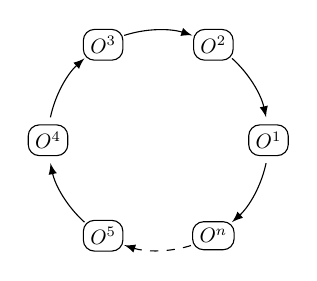
\begin{tikzpicture}[
circle/.style={
		scale=0.75,
		rounded corners,
		draw=black, 
		text centered,
		}
]

\def \n {6}
\def \m {4}
\def \radius {1.4cm}
\def \margin {12} % margin in angles, depends on the radius

\foreach \s in {1,...,\m}
{
  \node[draw, circle] at ({360/\n * (\s - 1)}:\radius) {$O^\s$};
  \draw[<-, >=latex] ({360/\n * (\s - 1)+\margin}:\radius) 
    arc ({360/\n * (\s - 1)+\margin}:{360/\n * (\s)-\margin}:\radius);
}

\node[draw, circle] at ({360/\n * 4}:\radius) {$O^5$};
  \draw[<-, dashed, >=latex] ({360/\n * 4+\margin}:\radius) 
    arc ({360/\n * 4+\margin}:{360/\n * (5)-\margin}:\radius);
    
\node[draw, circle] at ({360/\n * 5}:\radius) {$O^n$};
  \draw[<-, >=latex] ({360/\n * 5+\margin}:\radius) 
    arc ({360/\n * 5+\margin}:{360/\n * (6)-\margin}:\radius);


\end{tikzpicture}
\caption{링 정산}
\label{fig:settlement}
\end{figurehere}
\end{center}

트랜잭션을 만들기 위해 LPSC는 \verb|TokenTransferDelegate| 스마트 계약을 사용합니다. delegate 도입으로 인해 프로토콜 스마트 계약 업그레이드가 쉬워졌습니다. 모든 주문은 다른 프로토콜 버전을 적용하는 대신 delegate를 인가하기만 하면 프로토콜을 업그레이드할 수 있기 때문입니다.

주문-링 안의 각 주문을 위해, \verb|tokenS|의 결제는 구현에 따라 다음 번 또는 이전 주문에서 이루어집니다. 그리고, 링-채굴자가 선택한 수수료 모델에 따라 링-채굴자의 수수료가 지급됩니다. 마지막으로 모든 트랜잭션이 완료된 후에는 \verb|RingMined| 이벤트가 발생합니다.  

\subsubsection{발생한 이벤트\label{sec:events}}
프로토콜은 relay, 주문 브라우저, 가능한 효과적으로 주문 집계장 업데이트를 수신하기 위한 기타 행위자와 관련된 이벤트를 발생시킵니다. 발생한 이벤트 종류는 다음과 같습니다:

\begin{itemize}
	\item \textbf{OrderCancelled}: 특정 주문이 취소되었습니다.
	\item \textbf{OrdersCancelled}: 소유한 주소의 1개 페어 거래에 대한 모든 주문이 취소되었습니다.
	\item \textbf{AllOrdersCancelled}: 소유한 주소의 모든 페어 거래에 대한 모든 주문이 취소되었습니다.
	\item \textbf{RingMined}: 주문-링이 성공적으로 정산되었습니다. 이 이벤트는 각 내부-링 토큰 이체와 관련된 데이터를 담고 있습니다.
\end{itemize}


\section{LRx 토큰\label{sec:token}}
LRx는 우리의 토큰에 대한 일반적인 표기법입니다. LRC는 이더리움 기반 루프링 토큰이고, LRQ는 퀀텀(Qtum), LRN은 네오(NEO)입니다. 다음에 다른 블록체인들 기반으로 루프링이 배포되면 LRx 타입이 추가될 것입니다.

\subsection{수수료 모델\label{sec:fee_model}}
링-채굴자는 사용자에게 마진을 요청할 수 있으며 사용자는 주문을 생성할 때, 링-채굴자에게 수수료로 지급할 LRx 수량과 함께 주문에서 발생한 마진에 대한 비율(\verb|marginSplitPercentage|)을 지정합니다. 이것을 마진 분할(margin split)이라고 부릅니다. 수수료와 마진 분할 중 어떤 것을 선택할지는 링-채굴자가 결정합니다.   

아래는 마진 분할을 나타낸 것입니다:

\begin{center}
\begin{figurehere}
\centering
\begin{tikzpicture}[
scale=1,
font=\bfseries\footnotesize\sffamily,
classical/.style={thick,<->,shorten >=2pt,shorten <=2pt,>=stealth},
oneway/.style={->,dashed,shorten >=2pt,shorten <=2pt,>=stealth}
]
% Draw axes
\draw [->,thick] (0,1) node (yaxis) [above] {$$}
|- (6.2,0) node (xaxis) [right] {$$};

\draw
(4,0) coordinate (A)
(4,1) coordinate (A2)
(4.8,-0.6) coordinate (B)
(4.8,1) coordinate (B2)
(6,-0.6) coordinate (C)
(6,1) coordinate (C2);

\fill [draw=none, fill=gray!20] 
(4.8, 0) rectangle (6, 1);

\fill [draw=none, fill=gray!10] 
(0, -0.6) rectangle (4.8, 0);
\draw[thick] (0, -0.6) -- (0, 0.6) node[below]{$$};
\draw[thick, thin] (A) -- (A2) node[below]{$$};
\draw[thick, thin] (B) -- (B2) node[below]{$$};
\draw[thick] (C) node[below, xshift=0.5cm]{총 매수 수량} -- (C2) ;

\draw[classical] (0, 0.5) -> (4, 0.5) node[below]{$$};
\draw[classical] (4, 0.75) -> (4.8, 0.75) node[below]{$$};
\draw[classical] (4, 0.25) -> (6, 0.25) node[below]{$$};

\draw[oneway] (2, 1.2) node[above]{원래 주문의 매수 수량} -- (2, 0.5);
\draw[oneway] (4.4, 2.2) node[above]{추가 매수 수량} -- (4.4, 0.75);
\draw[oneway] (5.4, 1.6) node[above]{마진 분할} -- (5.4, 1);
\draw[oneway] (5, -1.2) node[below]{마진} -- (5, 0.25);
\draw[oneway] (2.4, -1.2) node[below]{주문에서 실제로 매수한 수량} -- (2.4, -0.5);
\end{tikzpicture}

\captionof{figure}{60\% 마진 분할}
\label{fig:marginsplit}
\end{figurehere}
\end{center}

주문-링의 마진이 너무 작다면 링-채굴자는 LRx 수수료를 선택할 것입니다. 반대로, 마진 분할 결과로 얻는 마진이 상당해서 LRx 수수료보다 훨씬 가치가 있다면, 링-채굴자는 마진 분할을 선택할 것입니다. 하지만 다른 조건이 필요합니다: 링-채굴자가 마진 분할을 선택하면, 그들은 사용자(주문 생성자)에게 수수료를 지급해야 하며, 이 수수료는 사용자가 링-채굴자에게 수수료로 지급했던 LRx와 같은 양입니다. 이것은 주문에 대한 LRx 수수료 2배 수준으로 링-채굴자가 마진 분할을 선택하는 경우에 대한 임계치(threshold)를 증가시키고, LRx 수수료를 선택하는 경향을 증가시킵니다. 이로 인해, 채굴자는 더욱 높은 마진 주문-링에서 많은 수익을 올리지 못하는 대신 낮은 마진 주문-링에서 지속적인 수익을 올리게 됩니다. 우리의 수수료 모델은 시장이 성장하고 완숙 단계에 접어들면 높은 마진 주문-링이 거의 없어질 것이고, 인센티브로 고정된 LRx 수수료가 필요하다는 기대를 기반으로 합니다.  

수수료는 결국 아래 그래프와 같은 모습이 될 것입니다:

\begin{center}
\begin{figurehere}
\centering
\begin{tikzpicture}[
font=\bfseries\footnotesize\sffamily,
oneway/.style={->,dashed,shorten >=2pt,shorten <=2pt,>=stealth},
scale=1]
% Draw axes
\draw [<->,thick] (0,2.7) node (yaxis) [above] {$y$}
|- (5,0) node (xaxis) [right] {$x$};

\draw
(1,1) coordinate (A)
(2,1) coordinate (B);


\draw[thick] (B) -- (3.7,2.7);
\draw[dotted] (B) -- (2,0) node[below] {$2f$};
\draw[dotted] (A) -- (1,0) node[below] {$f$};
\draw[thick,color=gray!70] (0,0) -- (2.7,2.7);
\draw[thick] (0,1) node[left] {$f$}--(B) node[     ]{$$};
\draw[oneway] (4,1) node[right]{예상 채굴 수익} -- (3, 2);


\end{tikzpicture}
\captionof{figure}{루프링 수수료 모델}
\label{fig:feemodel}
\end{figurehere}
\end{center}

$f$는 LRx 수수료, $x$는 마진 분할, $y$는 채굴 수익입니다. $y=max(f, x-f)$ 이며 실선으로 표시되었습니다; 주문에 대한 LRx 수수료가 $0$이면, 방정식은 $y=max(0, x - 0)$이 되고, 간단히 하면 $y=x$ 이며 회색 선으로 표시되어 있습니다.


그 결과는 다음과 같습니다:  
\begin{enumerate}
	\item 마진 분할이 0 이면, 링-채굴자는 고정된 LRx 수수료를 선택할 것이며, 여전히 인센티브를 받습니다. 
	\item LRx 수수료가 0 이면, 결과는 회색 선이며 수익은 일반적인 선형 모델을 기반으로 합니다.
	\item 마진 분할 수익이 2x(LRx 수수료) 보다 크면, 링-채굴자는 마진 수수료를 선택하고 사용자에게 LRx를 지급합니다.
\end{enumerate}

LRx 수수료가 0이 아니라면 링-채굴자가 어떤 선택을 하든지 상관없이 링-채굴자와 주문 생성자 사이에 LRx 이체가 항상 발생할 것이라는 점을 명심하시길 바랍니다. 링-채굴자는 LRx 수수료를 수익으로 올리거나, LRx 수수료를 주문 생성자에게 돌려주고 마진 분할을 선택합니다. 

링-채굴자는 수수료 일부를 지갑과 공유할 것입니다. 사용자가 지갑을 통해 주문을 내고 주문이 체결되면, 수수료 또는 마진 분할의 일부분이 지갑에게 보상으로 지급됩니다. 이것은 모듈 방식이고, 고유 비즈니스 모델 또는 구현을 통해 가능한 것입니다. 우리의 의도는 발생한 수익의 약 20\%-25\% 정도를 지갑이 가져가는 것입니다. 지갑은 사용자 기반을 가지고 있기 때문에 루프링 프로토콜 통합을 위한 주요 타깃(target)이지만 수입 원천이 없거나 미약합니다.   


\subsection{분권형 거버넌스}
근본적으로 루프링 프로토콜은 목표를 효과적으로 달성하기 위해 구성원 간의 협업(coordination)을 기반으로 하는 소셜 프로토콜입니다. 이 점은 일반적인 암호 경제 프로토콜과 유사하며, 그 유용성은 주로 합동 문제 \cite{vitalikgovernance}, 무자비한 보복 균형(grim trigger equilibrium), 제한된 합리성(bounded rationality)과 동일한 메커니즘에 의해 보호받습니다. 이를 위해 LRx 토큰은 수수료를 지급하는데 사용할 뿐만 아니라 다양한 네트워크 참여자에 대한 재정적인 인센티브를 조정하는(align) 용도로 사용됩니다. 이러한 조정은 광범위한 채택을 위해 모든 프로토콜에서 필요한 것이지만, 견고한 분권형 생태계에서 유동성을 개선하는 것이 성공의 지표가 되는 거래소 프로토콜에서는 더욱 중요한 요소입니다.  

LRx 토큰은 분권형 거버넌스를 통해 프로토콜 업데이트를 완료하는데 사용될 수 있을 것입니다. 지속성과 보안성을 보장하고 비호환성(incompatibility)으로 인해 발생하는 유동성 리스크를 줄이기 위해, 스마트 계약 업데이트는 토큰 보유자에 의해 운영될 것입니다. 스마트 계약이 배포된 이후에도 교체되지 않았을 경우, dApp 이나 사용자는 이제는 사용하지 않는(deprecated) 버전과 상호 작용을 계속하고, 업데이트된 계약에서 그들이 제외될 위험이 있습니다. 근원 블록체인에 적용하고 시장 요구를 반영해야 하므로, 업그레이드 지원은 프로토콜의 성공에 있어 중요한 요소입니다. LRx 이해당사자(stakeholders)에 의한 분권형 거버넌스는 dApp 이나 사용자에게 지장을 주지 않고, 또는 스마트 계약 추상화(abstraction)에 과도하게 의존하지 않고도 프로토콜 스마트 계약을 업데이트할 수 있을 것입니다. LRx 토큰의 공급은 고정적이며, LRC의 경우 루프링 재단이 일정 비율을 동결했으며, 커뮤니티 기금\cite{LRCtokendoc}으로 할당했습니다. 

하지만, 프로토콜의 방향을 이끌 이해당사자로 고려하는 대상이 LRx 토큰 소유자만 있는 것은 아닙니다: relay/링-채굴자, 지갑, 개발자 및 기타 생태계 구성 요소 등도 있으며, 이들의 목소리도 들어봐야 합니다. 실제로, 이러한 에이전트들이 각자의 업무를 수행하기 위해 LRx를 보유할 필요가 없다는 점을 고려했을 때(전통적인 maker/taker, 시장 조성자가 존재하지 않기 때문에 초기 토큰 준비는 불필요함), 우리는 그들의 소중한 관심에 대해 대체 수단을 마련해야 합니다. 그뿐만 아니라, "간단한" 토큰 기반 투표는 온 체인과 오프 체인 모두 낮은 투표율, 토큰 소유권 집중으로 인한 위험성과 같은 문제가 있기 때문에 의견 불일치에 대한 불완전한 해결책일 뿐입니다. 따라서, 거버넌스 모델의 구현 목표는 계층 구조이며, 의사 결정 과정의 일부가 표준(norm)이 되는 공유 지식을 기초로 합니다. 협업 단체가 이런 업무를 원활히 진행할 수 있으며 다양한 참여자의 의사와 개발 중인 프로토콜의 주요 사안을 제공할 수 있을 것입니다. 이것이 실현되면, 루프링 재단은 필연적으로 프로토콜 개발자에서 프로토콜 관리자(stewards)로 진화할 것입니다.    

\section{사기와 공격 보호}

\subsection{선행-매매 방지\label{sec:dual_authoring}}

분권형 거래소에서 선행매매는 누군가가 다른 노드의 거래 솔루션을 모방해서, 보류 중인(pending) 트랜잭션 풀(mempool) 안에 있는 원래의 트랜잭션보다 먼저 채굴하는 것을 말합니다. 다른 사람보다 높은 트랜잭션 수수료(가스 가격)를 지정해서 선행매매를 성공시킬 수 있습니다. 루프링(주문-매칭 관련 모든 프로토콜 포함)에서 주로 시도되는 선행매매 형태는 주문-훔치기(order-filch)입니다: 선행매매자가 보류 중인 주문-링 정산 트랜잭션에서 1개 이상의 주문을 훔친 경우; 루프링에서만 발생하는 선행매매 형태도 있습니다: 선행매매자가 보류 중인 트랜잭션에서 전체 주문-링을 훔친 경우

submitRing 트랜잭션이 확정되지 않았고 아직 보류 중인 트랜잭션 풀에 있는 경우, 누구든지 이런 트랜잭션을 쉽게 찾을 수 있고, \verb|minerAddress|를 자신이 소유한 주소(the \verb|filcherAddress|)로 교체할 수 있습니다. 그리고 그들은 주문-링의 서명을 대체하기 위해 \verb|filcherAddress|를 이용해 페이로드(payload)를 다시 서명할 수 있습니다. 이러한 일을 계획한 사람(filcher)은 다른 사람보다 높은 가스 가격을 설정해 새로운 트랜잭션을 제출합니다. 이들은 본래의 submitRing 트랜잭션 대신 이들이 만든 새로운 트랜잭션을 블록-채굴자가 다음 번 블록에서 선택해주길 희망합니다.

이 문제에 대한 기존 해결책들은 중대한 단점이 있습니다: 추가적인 트랜잭션이 필요하기 때문에 링-채굴자에게 지급하는 가스 비용을 늘어납니다; 주문-링을 정산하려면 최소한 두 개의 블록이 필요합니다. 우리의 새로운 해결책인 듀얼 인가(Dual Authoring)\cite{dualauthor}는 정산과 링-채굴 두 단계(level)에서 주문 인가를 설정한 메커니즘을 담고 있습니다.

듀얼 인가 과정은 다음과 같습니다:

\begin{enumerate}

	\item 지갑 소프트웨어는 각 주문에 대해 공개키/개인키 페어를 무작위(random)로 생성할 것이며, 이 키 페어는 주문의 JSON 스니펫(snippet)에 추가될 것입니다. (바이트 사이즈를 줄이기 위해 공개키 자체를 사용하는 대신 공개키에서 파생된 주소를 사용하는 방법이 있습니다. 우리는 \verb|authAddr|로 이 주소를 표현하고 있으며, \verb|authAddr|과 매칭되는 개인키를 표현하기 위해 \verb|authKey|를 사용합니다).

	\item \verb|r|, \verb|v|, \verb|s|, \verb|authKey|를 제외한 주문에 있는 모든 필드로 주문의 해시를 계산하고, \verb|owner|의 개인키(\verb|authKey|가 아님)를 사용해 해시에 서명합니다.

	\item 지갑은 링-채굴을 위해 주문을 \verb|authKey|와 함께 relay에게 보낼 것입니다. 링-채굴자는 \verb|authKey|와 \verb|authAddr| 이 정확하게 일치하는 페어인지, \verb|owner| 주소와 관련해 주문의 서명이 유효한지 검증할 것입니다.

	\item 주문-링이 식별되면, 링-채굴자는 각 주문의 \verb|authKey|를 사용해 링의 해시와 모든 채굴 관련 매개변수에 서명할 것입니다. 주문-링에 $n$ 개 주문이 포함되어 있다면, $n$ 개의 \verb|authKey|에 의해 $n$ 개의 서명이 생성될 것입니다. 우리는 이 서명들을 \verb|authSignature|s라고 부릅니다. 링-채굴자는 \verb|minerAddress|의 개인 키를 사용해 모든 채굴 관련 매개변수와 링 해시에 서명해야 할 수도 있습니다.
 
	\item 링-채굴자는 \verb|authSignature|s 뿐만 아니라 모든 매개변수와 함께 submitRing 함수를 호출합니다. \verb|authKey|는 온-체인 트랜잭션의 일부가 아니며, 링-채굴자 자신 이외는 모르는 상태로 유지된다는 점을 명심하세요.

	\item 이제, 루프링 프로토콜은 각 주문의 \verb|authAddr|에 해당하는 각각의 \verb|authSignature|를 검증할 것이며, \verb|authSignature|가 없거나 유효하지 않은 경우 해당 주문-링을 거부(reject) 처리할 것입니다.
 
\end{enumerate}

지금까지 결과는 다음과 같습니다:

\begin{itemize}

	\item  주문의 서명(\verb|owner| 주소의 개인키로 서명한)은 \verb|authAddr|과 주문을 변경할 수 없다는 것을 보장합니다.
	\item  링-채굴자의 서명(\verb|minerAddress|의 개인키로 서명한)이 제공된 경우, 이 서명은 주문-링을 채굴하는데 그 누구도 해당 채굴자의 신원을 사용할 수 없다는 점을 보장합니다. 
	\item  \verb|authSignature|s는 \verb|minerAddress|와 전체 주문-링을 변경할 수 없고, 어떤 주문도 도난당할 수 없다는 점을 보장합니다. 

\end{itemize}

듀얼 인가는 단일 트랜잭션에서 주문-링 정산 수행을 보장하면서도 링-훔치기와 주문-훔치기를 방지합니다. 추가로, 듀얼 인가는 relay가 두 가지 방법으로 주문을 공유할 수 있는 길을 열어주었습니다: 매칭 가능한 주문과 매칭 불가능한 주문. 기본적으로 루프링은 OTC 모델로 운영하며, 지정자 주문만을 지원합니다. 즉, 주문의 타임스탬프는 무시됩니다. 이것은 선행매매가 실제 거래 가격에는 영향을 주지 못하며, 거래 실행 여부에만 영향을 준다는 것을 의미합니다.

\section{기타 공격}

\subsection{시빌 공격 또는 DOS 공격}
악의적인 사용자가 - 직접 또는 위조된 신원으로 활동하는 - 루프링 노드를 공격하기 위해 많은 양의 소액 주문들을 보낼 수 있습니다. 하지만, 노드는 자체 기준 - 기준은 숨기거나 공개할 수 있음 - 에 따라 주문을 거부할 수 있기 때문에, 이러한 형태의 주문 대부분은 주문이 매치되었을 때 만족스러운 수익을 올리지 못하도록 거부될 것입니다. relay에게 주문을 관리하는 방법을 결정할 수 있는 권한을 주었기 때문에, 우리는 대규모 소액 주문 공격을 위협으로 보지 않습니다.    

\subsection{불충분한 잔액}
악의적인 사용자가 주문 값이 0이 아니지만, 그곳의 주소에 있는 실제 잔액은 0인 주문들에 서명하고 퍼뜨릴 수 있습니다. 노드는 주문의 실제 잔액이 0인지 주의 깊게 모니터할 수 있으며, 이러한 주문이 발견되면 주문 상태를 업데이트하고 이들을 제거할 수 있습니다.
노드는 주문 상태를 업데이트하기 위해 시간을 투자해야 하며, 관련된 주문을 누락시키거나 주소 블랙리스트를 활용하는 방법 등을 통해 수고를 최소화할 방안을 모색할 수 있습니다.


\section{요약}

루프링 프로토콜은 분권형 거래소를 위한 기본적인 계층으로 출발했습니다. 그렇게 함으로써, 루프링 프로토콜은 사람들의 자산과 가치 교환 방법에 엄청난 영향을 주었습니다. 중간 상품으로서 돈은 물물 교환을 쉽게 하거나 대체하고, 두 거래 당사자가 상대방의 확실한 상품이나 서비스를 원해야 하는 필요의 이중 일치(double coincidence of wants) 문제\cite{unenumerated2006}를 해결합니다. 이와 유사하게, 루프링 프로토콜은 거래를 더욱 쉽게 성사시키는 링 매칭을 사용해 페어 거래 안에서 발생하는 필요의 일치에 대한 의존성을 없애는 것을 목표로 합니다. 토큰, 전통적인 자산 등을 사회와 시장에서 교환하는 방법과 관련해 이것은 의미 있는 일입니다. 실제로, 분권형 암호 화폐가 돈에 대한 국가의 통제에 위협이 되는 것처럼, 특정 규모에서 거래자(소비자/생산자)를 연결할 수 있는 조합 프로토콜은 돈 개념 자체에 대해 이론적으로 위협이 됩니다.  

프로토콜의 이점은 다음과 같습니다:

\begin{itemize}
	\item 오프-체인 주문 관리와 온-체인 정산은 보안을 위해 성능을 희생하지 않아도 된다는 점을 의미합니다.
	\item 링-채굴과 주문 공유를 통해 유동성이 증가합니다.
	\item 듀얼 인가는 현재 모든 DEX와 그들의 사용자가 겪고있는 치명적인 선행매매 문제를 해결합니다.
	\item 무료, 공개형 스마트 계약덕분에 프로토콜을 활용해 dApp을 만들거나 프로토콜과 dApp이 상호 작용할 수 있습니다.
	\item 운영자 간의 표준은 사용자 경험을 개선하고 네트워크 효과를 가져옵니다.
	\item 주문 집계장과 통신을 위해 운영되는 네트워크는 유연하게 유지됩니다.
	\item 낮아진 진입 장벽으로 인해 네트워크와 사용자를 연결하는 노드의 비용이 감소합니다. 
	\item 사용자 지갑에서 직접 익명 거래를 할 수 있습니다.
\end{itemize}

\section{감사의 글}

우리의 멘토, 고문, 그리고 그들의 지식을 기꺼이 제공하고 우리를 환대해준 커뮤니티의 많은 분들께 감사의 말을 전하고 싶습니다. 특히, Shuo Bai(ChinaLedger); Haibin Kan 교수님; Alex Cheng, Hongfei Da; Yin Cao; Xiaochuan Wu; Zhen Wang, Wei Yu, Nian Duan, Jun Xiao, Jiang Qian, Jiangxu Xiang, Yipeng Guo, Dahai Li, Kelvin Long, Huaxia Xia, Jun Ma, 그리고 이 프로젝트에 피드백을 제공하고 리뷰를 해준 Encephalo Path에게 감사드립니다.


\bibliography{whitepaper}
\bibliographystyle{unsrt}

%
\end{multicols}
%
%
%\begin{appendices}
%
%\section{EVM 환경에서 구현된 루프링\label{app:protocol_ethereum}}
%
%\begin{center}
%\begin{figurehere}
%\centering
%\begin{tikzpicture}
%[node distance = 1cm, auto,font=\footnotesize,
%% STYLES
%every node/.style={node distance=3cm},
%% The comment style is used to describe the characteristics of each force
%comment/.style={rectangle, inner sep= 5pt, text width=4cm, node distance=0.25cm, font=\scriptsize\sffamily},
%% The force style is used to draw the forces' name
%force/.style={rectangle, draw, fill=black!10, inner sep=5pt, text width=4cm, text badly centered, minimum height=1.2cm, font=\bfseries\footnotesize\sffamily}] 
%
%% Draw forces
%\node [force] (impl) {LoopringProtocolImpl};
%\node [force, dashed, above of=impl] (protocol_interface) {LoopringProtocol};
%\node [force, left=1cm of impl] (nameregistry) {NameRegistry};
%\node [force, right=1cm of impl] (tokenregistry) {TokenRegistry};
%\node [force, below of=impl] (delegate) {TokenTransferDelegate};
%\node [force, left=1cm of delegate] (multisig) {TransferableMultsig};
%
%%%%%%%%%%%%%%%%
%% Change data from here
%
%% impl
%\node [comment, below=0.25 of impl] (comment-impl) {- 주문-링 유효성 검증\\
%- 정산을 위한 토큰 이체\\
%- 이벤트 발생};
%
%% nameregistry
%\node [comment, below=0.25cm of nameregistry]{- 지갑과 relay 등록};
%
%% protocol_interface
%\node [comment, below=0.25 of protocol_interface](comment-interface) {- 인터페이스와 이벤트 정의};
%
%% tokenregistry
%\node [comment, below=0.25 of tokenregistry] {- ERC20/ERC223 토큰 등록};
%
%% delegate
%\node [comment, below=0.25 of delegate] {- 사용자를 대신해 토큰 이체};
%
%% PUBLIC POLICIES
%\node [comment, text width=3cm, below=0.25 of multisig] {- 다중 서명 소유권 활성화};
%
%%%%%%%%%%%%%%%%%
%
%% Draw the links between forces
%\path[->,thick] 
%(comment-interface) edge (impl)
%(nameregistry) edge (impl)
%(tokenregistry) edge (impl)
%(delegate) edge (comment-impl);
%
%\end{tikzpicture} 
%\caption{스마트 계약}
%\label{fig:smartcontracts}
%\end{figurehere}
%\end{center}
%
%\section{Deployment}
%
%
%\subsection{Ethereum}
%아래의 스마트 계약은 이더리움 메인넷에 배포되었습니다:
%\begin{itemize}
%\item LRC: \verb|0xEF68e7C694F40c8202821eDF525dE3782458639f|
%\item TokenRegistry: \verb|0xa21c1f2AE7f721aE77b1204A4f0811c642638da9|
%\item TokenTransferDelegate: \verb|0x7b126ab811f278f288bf1d62d47334351dA20d1d|
%\item NameRegistry: \verb|0xd181c1808e3f010F0F0aABc6Fe1bcE2025DB7Bb7|
%\item LoopringProtocolImpl: \verb|0x0B48b747436f10c846696e889e66425e05CD740f|
%\end{itemize}
%
%\subsection{Qtum}
%아래의 스마트 계약은 퀀텀 메인넷에 배포되었습니다:
%\begin{itemize}
%\item LRQ: \verb| 2eb2a66afd4e465fb06d8b71f30fb1b93e18788d |
%\item TokenRegistry: \verb| c89ea34360258917daf3655f8bec5550923509b3 |
%\item TokenTransferDelegate: \verb| 60b3fa7f461664e4dafb621a36ac2722cc680f10 |
%\item NameRegistry: \verb| e26a27d92181069b25bc7283e03722f6ce7678bb |
%\item LoopringProtocolImpl: \verb| 5180bb56b696d16635abd8dc235e0ee432abf25d |
%\end{itemize}
%
%\end{appendices}
\end{document}
